%%%%%%%%%%%%%%%%%%%%%%%%%%%%%%%%%%%%%%%%%%%%%%%%%%%%%%
%
% This file defines the style for your report
% You don't need to edit it any more, if not to change the authors name.
%
% Search below for the keyword:   GROUP
% insert your group number
%
% Search below for the keyword:   AUTHORS
% insert the name of the authors
%
% If you want to compile your document you have TWO ways
% depending on the fact that 
% 	1) you have inserted only postscript images in your .tex file 
%		---> then go to MODE 1
%	2) you have inserted other kind of images (jpg, pdf, ...) in your .tex file
%		---> then go to MODE 2
%
% MODE 1 
% Type:
% 	latex homebook.tex
%
% If the compilation runs successfully and you want to see the results type:
% 	xdvi homebook.dvi &
% and use the menus to go through the document
%
% If you want to create a pdf type:
% 	dvipdfm homebook.dvi
%
% a homebook.pdf file is created
% you can see it using the command:
% 	acroread homebook.pdf &
%
%
% MODE 2
% Type:
%	pdflatex homebook.tex
%
% If the compilation runs successfully you directly have the pdf file
% and you can see it using the command:
%       acroread homebook.pdf &
%
% 
%%%%%%%%%%%%%%%%%%%%%%%%%%%%%%%%%%%%%%%%%%%%%%%%%%%%%%

\documentclass[11pt, english, makeidx, a4paper, titlepage, oneside]{book}
\usepackage{babel}
\usepackage{fancyhdr}
\usepackage{makeidx}
\usepackage{titlesec}
\usepackage{listings}
\usepackage{booktabs}
\usepackage{wrapfig}

\newenvironment{listato}{\footnotesize}{\normalsize }

%\pagestyle{empty}

\textwidth 15.5cm
\textheight 23 cm
\topmargin -1cm
\oddsidemargin -0.5cm
\linespread{1.2}

\pagestyle{fancy}
\lhead{}
\chead{Microelectronic Systems}
\lfoot{}
\cfoot{}
\rfoot{}
\rhead{\thepage}

\usepackage{graphicx}
\usepackage{amsmath}
\usepackage{amsfonts}
\usepackage{amsthm}
\usepackage{amssymb}
%\oddsidemargin -1.1cm
\usepackage{graphicx}
\usepackage{caption}
\usepackage{float}
\usepackage{amsmath}
\usepackage{amssymb}
\usepackage{amsfonts}
\usepackage{xcolor}
\usepackage{amsthm}
%\usepackage{subscript}
\usepackage{empheq}
\usepackage{datetime}
\usepackage{verbatim}
\usepackage{listings}
\usepackage{fancyvrb}

\definecolor{mGreen}{rgb}{0,0.6,0}
\definecolor{mGray}{rgb}{0.5,0.5,0.5}
\definecolor{mPurple}{rgb}{0.58,0,0.82}
\definecolor{backgroundColour}{rgb}{0.95,0.95,0.92}


\lstdefinestyle{B}{
	backgroundcolor=\color{backgroundColour},   
	commentstyle=\color{mGreen},
	keywordstyle=\color{magenta},
	numberstyle=\tiny\color{mGray},
	stringstyle=\color{mPurple},
	basicstyle=\ttfamily,
	breakatwhitespace=false,         
	breaklines=true,                 
	captionpos=b,                    
	keepspaces=true,                 
	numbers=none,                    
	numbersep=5pt,                  
	showspaces=false,                
	showstringspaces=false,
	showtabs=false,                  
	tabsize=2,
	language=bash,
	keepspaces=true,
	columns=flexible
}



\newdate{discussion}{31}{10}{2018}
\newcommand{\pc}{\textit{PC }}
\newcommand{\alu}{\textit{ALU }}
\newcommand{\rf}{\textsf{RF }}
\newcommand{\dlx}{\textit{DLX }}

\lstdefinelanguage{VHDL}{morekeywords={library,use,all,entity,generic, is,port,in,out,end,architecture,of,begin,and,if,then,else,elsif,process},morecomment=[l]--}

\lstdefinestyle{vhdl}{language = VHDL, basicstyle = \ttfamily, keywordstyle = \color{keyword}\bfseries, commentstyle = \color{comment}}

\titleformat{\chapter}[display]
{\normalfont\Large\filcenter\sffamily}
{\titlerule[0.5pt]%
\vspace{1pt}
\titlerule
\vspace{1pc}
\LARGE\MakeUppercase{\chaptertitlename} \thechapter
}
{1pc}
{\titlerule
\vspace{1pc}
\Huge}

\makeindex

\begin{document}

\frontmatter
\begin{titlepage}
\vspace{0cm}
\centerline{

\includegraphics[width=3cm]{./logopoli}} 
\vspace{0.5cm}
\centerline{\LARGE Politecnico di Torino}
\vspace{2.5cm}
\centerline{\huge\sf Microelectronic Systems}
\vspace{1cm}
\centerline{\Huge\sf DLX Microprocessor: Design \& Development}
\bigskip
\centerline{\huge\sf Final Project Report}
\vspace{2cm}
\centerline{\Large Master degree in Electronics Engineering}
\vspace{4.5cm}
%%%%%%%%%%%%%%%%%%%%%%%%%%%%%%%%%%%%%%%%%%%%%%%%%%%%%%
\centerline{\large Referents: Prof. Mariagrazia Graziano, Giovanna Turvani}
\bigskip
\vspace{1cm}
%%%%%%%%%%%%%%%%%%%%%%%%%%%%%%%%%%%%%%%%%%%%%%%%%%%%%%
% GROUP
\centerline{\large Authors: Group 15}
\bigskip
%%%%%%%%%%%%%%%%%%%%%%%%%%%%%%%%%%%%%%%%%%%%%%%%%%%%%%
% AUTHORS
\centerline{\large Alberto Anselmo, Giulio Roggero}
%%%%%%%%%%%%%%%%%%%%%%%%%%%%%%%%%%%%%%%%%%%%%%%%%%%%%%
\vspace{2cm}
\centerline{\large \displaydate{discussion}}
\end{titlepage}

\tableofcontents

\mainmatter
%%%%%%%%%%%%%%%%%%%%%%%%%%%%%%%%%%%%%%%%%%%%%%%%%%%%%%
% Chapters
%% Introduction
%%%%%%%%%%%%%%%%%%%%%%%%%%%%%%%%%%%%%%%%%%%%%%%%%%%%
%\graphicspath{chapters/figures/}
\chapter{Presentation}
\label{chap_intro}

%%%%%%%%%%%%%%%%%%%%%%%%%%%%%%%%%%%%%%%%%%%%%%%%%%%%%%%%%%%
In this brief overall presentation, we will just summarize the main design choices we have made for the development of our project. 

\paragraph{Instruction Set}
The first thing to be noticed is that we have decided to implement all the possible instructions that were included in the set assigned, except for the floating point operations, which would have lowered down a lot the maximum operating frequency, if not pipelined in more stages.

\paragraph{Design}
Following the required specifications, we have added to our processor, piece by piece, all the components needed to perform the operations. The approach we followed was to try to reuse most of the work already done for the laboratories, since its behavior was well-known and already tested. On the other hand, for some units, we had to start from scratches, since they were not involved in any previous activities.

\paragraph{Control Unit}
For this part, we decided that the most suitable approach for our project was the \textit{FSM} version, since it gave us enough flexibility to implement all the instructions without the need to stall for too many cycles the pipeline. At the same time, we thought it was less complex to deal with than the micro programmed control unit.

\paragraph{Additional features}
After having finished with the previous points, we decided to include \textit{Dynamic Branch Prediction} and \textit{Data Forwarding} as additional features for our processor. In particular, a \textit{Branch History Table} has been added to the \textit{Fetch} stage and some additional signals now bypass some registers, when needed.

\paragraph{Synthesis}
Finally, the whole processor has been synthesized using the script provided in appendix \textbf{ADDDDDDDDDDDDDDDDDDDDDDDDDDDDDDDDDDDDDDDDD HERE}


%% Datapath chapter
\chapter{Datapath}
%%%%%%%%%%%%%%%%%%%%%%%%%%%%%%%%%%%%%%%%%%%%%%%%%%%%
%\graphicspath{chapters/figures/}
\section{Fetch Stage}
\label{chap_ft}

%%%%%%%%%%%%%%%%%%%%%%%%%%%%%%%%%%%%%%%%%%%%%%%%%%%%%%%%%%%
\subsection{Introduction}
The fetch stage is important to provide to our processor a new instruction at every clock cycle, if needed. It is the first stage that a function actually enters in its execution flow.

Here are presented the signals involved:
\begin{itemize}
	\item \textit{CLK} is the usual clock signal needed to synchronize the system
	\item \textit{STALL} is a control signal, that blocks the update of the \textsf{PC} and therefore does not let any other operations to be issued
	\item \textit{RST} it's the canonical reset signal
	\item \textit{RST\_DEC} \textbf{ALBI PLEASE ADD EXPLANATION HERE}
	\item \textit{PC\_SEL} is a control signal which selects the next value of the \textit{PC}, either from the normal execution flow or from the ALU
	\item \textit{JB\_INST} is the computed new \textit{PC} value coming from the \alu
	\item \textit{FUNC} is a part of the instruction, for the \textsc{R\_TYPE} operations
	\item \textit{OPCODE} represents the type of operation in the instruction set to be performed by the processor
	\item \textit{NPC} which is the canonical updated \pc, pointing to the next instruction
	\item \textit{INST\_OUT} is a signal that comes from the IRAM, after the instruction has been read
	\item \textit{MISS\_HIT} is used to inform the system whether the prediction made was correct or not
	\item \textit{FLUSH\_CTL} is a control signal which allows us to clean the pipe in case of a wrong prediction
\end{itemize}

\subsection{Main units}
There are several instances we decided to use in this stage. The main ones are reported below.
\paragraph{Branch predictor}
The purpose of this unit is to give a reliable dynamic prediction regarding the behaviour of a branch before its correct target address is computed. More details can be found in a dedicated section \ref{dyn_br}.
\paragraph{IRAM}
It is the instruction memory, where the operations that have to be executed are stored. It is addressed by the \pc.
\paragraph{Registers}
There are several registers that are actually used to store the values of:
\begin{itemize}
	\item \textit{PC} counter, current and next value
	\item \textit{INSTR} which saves the instruction fetched from the \textsf{IRAM}
	\item \textit{TMP\_RST}, where the reset signal is sampled in order to synchronize the reset phase
\end{itemize}
\paragraph{Mux}
This unit is used here to selected the correct value of the next \pc: either the one coming from the memory or the following instruction, following the normal execution flow.
\paragraph{Adder}
This very simple unit just provides the $+4$ value for the new \pc.
%%%%%%%%%%%%%%%%%%%%%%%%%%%%%%%%%%%%%%%%%%%%%%%%%%%%
%\graphicspath{chapters/figures/}
\section{Decode Stage}
\label{chap_dec}

%%%%%%%%%%%%%%%%%%%%%%%%%%%%%%%%%%%%%%%%%%%%%%%%%%%%%%%%%%%
\subsection{Introduction}
The decode stage is the second one. Here the instructions stored in the \textit{IRAM} that have been previously read are decomposed in order to correctly identify all the information regarding the operation that will be performed. In this way, we can read the correct source, target and destination address, as well as the immediate values. Moreover, also the \textsf{OPCODE}, which represents the particular instruction to be executed, is read.

The most relevant signals involved in this stage are:
\begin{itemize}
	\item \textit{FLUSH} is a control signal, which is necessary to clean the pipe
	\item \textit{}
	\item \textit{}
	\item \textit{}
	\item \textit{}
	\item \textit{}
	\item \textit{}
	\item \textit{}
	\item \textit{}
	\item \textit{}
	\item \textit{}
	\item \textit{}
	\item \textit{}
	\item \textit{}
	\item \textit{}
	\item \textit{}
	\item \textit{}
	\item \textit{A,B,C,D} are the outputs, storing the values coming from the \textsf{RF} and the two immediate values
	\item \textit{RT, RS} are the addresses of the target and source address respectively, which are needed to implement the data forwarding
	\item \textit{DEST\_OUT} is the address for the final commit during the write back stage
\end{itemize}

%FLUSH :   IN std_logic;
%DATAIN :  IN std_logic_vector(NB-1 downto 0);
%IMM1 :    IN std_logic_vector(NB-7 downto 0);
%IMM2 :    IN std_logic_vector(NB-1 downto 0);
%BR_TYPE : IN std_logic_vector(1 downto 0);
%JMP :     IN std_logic;
%RI:       IN std_logic;
%US :      IN std_logic;
%RD1:      IN std_logic;
%RD2:      IN std_logic;
%WR:       IN std_logic;
%ADD_WR:   IN std_logic_vector(LS-1 downto 0); 
%ADD_RD1:  IN std_logic_vector(LS-1 downto 0);
%ADD_RD2:  IN std_logic_vector(LS-1 downto 0);
%DEST_IN : IN std_logic_vector(LS-1 downto 0);
%HAZARD:   OUT std_logic;
%US_TO_EX: OUT std_logic;
%%%%%%%%%%%%%%%%%%%%%%%%%%%%%%%%%%%%%%%%%%%%%%%%%%%%
%\graphicspath{chapters/figures/}
\chapter{Execution Unit}
\label{chap_exu}

%%%%%%%%%%%%%%%%%%%%%%%%%%%%%%%%%%%%%%%%%%%%%%%%%%%%%%%%%%%
\section{Overview}
We have designed an execution unit that is capable of dealing with almost all the instructions present in the instruction set that has been given. Exceptions are the floating point operations, which requires speicific hardware that we decided not to include. It is worth mentioning that normally the \textit{MUL} operations are executed by dividing them in subsequently pipelined stages. Here, differently, in order to keep the 5 stages in the pipeline and not to alter the normal execution flow, this doe not take place. As a consequence, the maximum operating frequency will be heavily affected by the propagation time needed by the multiplier to finish its job.


In the \textit{Execution Unit} are therefore present the following components:
\begin{itemize}
	\item \textbf{shifter}, used in order to shift and rotate the value contained in an input register
	\item \textbf{adder}, necessary obviously to perform addition and subtraction between values, but also used in the logic comparison operations
	\item \textbf{logic}, unit to perform logic bitwise operations, such as \textit{OR, AND, XOR} and so on
	\item \textbf{comparator}, which purpose is to determine whether an input is greater, smaller or equal than another one
	\item \textbf{multiplier}, whose goal is to perform multiplications between inputs
	\item \text{PC adder}, a dedicated adder to increase by the value of the PC, useful in case of a \textit{JMP} operation
	\item \textbf{registers}, to update the inputs and store the results
	\item \textbf{muxes}, to select the results coming from the required unit and correctly update the outputs of the stage
	\item \textbf{inverter}, needed to perform the \textit{2'S complement} and perform the subtraction
\end{itemize}


For this stage, a bunch of bits of the \textsf{CW} are used. Here are reported:
\begin{itemize}
	\item \textit{ENEX}, a general enable for the components and especially for the registers
	\item \textit{MUX1\_SEL}, a selection signal for the mux that is able to select an immediate value or a register an input that as the first term for the other units
	\item \textit{MUX2\_SEL}, with a goal similar as the one above, but for the second input
	\item \textit{UN\_SEL}, 3 bits signal that selects the correct input, which is then sent to a register
	\item \textit{OP\_SEL}, 4 bits selection signal, used to indicate to each unit, with different encoding, the operation to be performed
	\item \textit{PC\_SEL}, selection signal to update the PC counter correctly, following a branch or jump.
\end{itemize}


\section{Adder}

For the adder architecture, we decided not to start from scratches. As long as our P4 adder, designed during the laboratories, has a general description, we resized it to our architecture on 32 bits. This means that we have included the components capable of producing the \textsf{PG} propagate and generate signals and the \textsc{G} ones used to produce only the generate and so the final carry. We consider that therefore the result, in terms of performance can satisfy us. At the input of the block, we have also a \textit{C\_IN} signal, which is used to create, in cooperation with the inverter, the \text{2'S complement} of the input used (either immediate or coming from a register), in order to produce as a final result the signed sum. There are few control signals used for this unit. In figure \ref{adder_fig} is presented the simple schematic of the adder block.

\begin{figure}
	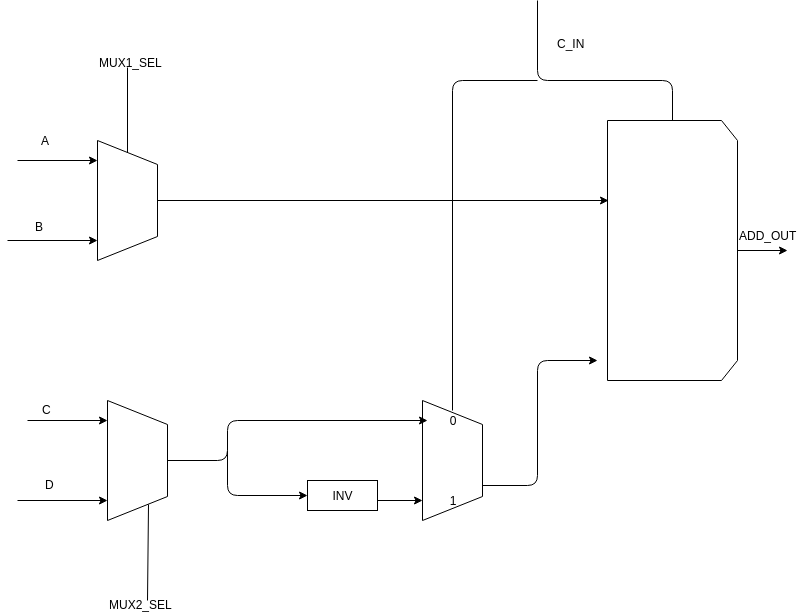
\includegraphics[width=\textwidth]{chapters/figures/adder}
	%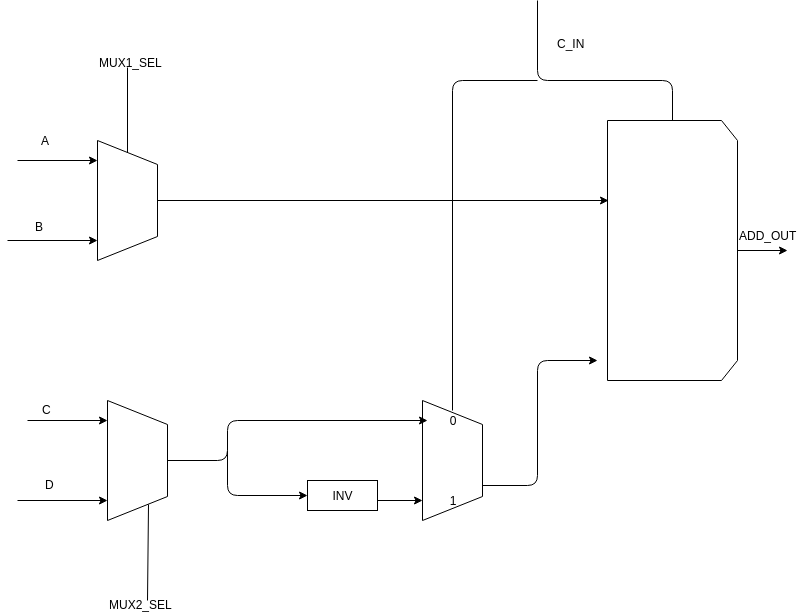
\includegraphics[width=\textwidth]{chapters/figures/adder}
	\caption{Adder with inverter and related selection signal}
	\label{adder_fig}
\end{figure}


\section{Logic}

In order to perform some logic bitwise operations, we have reproduced the microarchitecture that has been used for the \textsf{T2}. Here, in figure \ref{logic_fig} is briefly reported the gates needed, that combined between each other, are capable of giving us the desired operations, as reported in the table \ref{logicT2_table}.

\begin{table}[ht]
	\centering
	\begin{tabular}{c|cccc}
		\toprule
				& S0 	& S1	& S2	& S3 \\
		\midrule
		AND		& 0		& 0		& 0		& 1	 \\
		NAND	& 1		& 1		& 1		& 0	 \\
		OR		& 0		& 1		& 1		& 0	 \\
		NOR		& 1		& 0		& 0		& 0	 \\
		XOR		& 0		& 1		& 1		& 0	 \\
		XNOR	& 1		& 0		& 0		& 1	 \\
		\bottomrule
	\end{tabular}
	\caption{Combination of control signal for logic operations}
	\label{logicT2_table} % here is the table label
\end{table}

The control signal \textit{S} is required to be on 4 bits: for this reason, we have implemented in our control word 4 bits for this purpose. In particular, the signal \textsf{OP\_SEL} plays this role. We could have used 3 bits on the \textit{CW} and design an encoder, but the savings in term of connection would have been ruined by the need of an additional decoder. Moreover, these bits are not switched most of the time, thus providing a not so relevant switching power dissipation.

\begin{figure}
	\centering
	%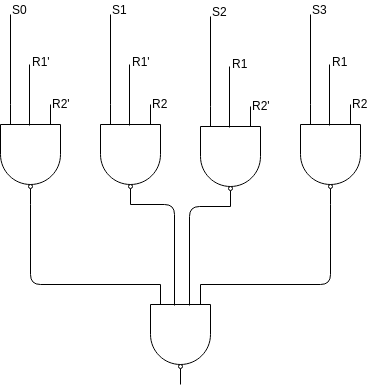
\includegraphics[width=\textwidth]{chapters/figures/logicT2}
	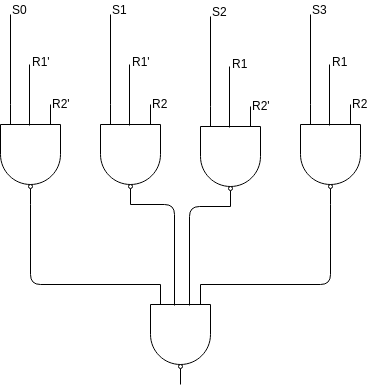
\includegraphics[scale=0.6]{chapters/figures/logicT2}
	\caption{T2 logic for a single bit}
	\label{logic_fig}
\end{figure}

\section{Shifter}

To define the lateral shifts, left or right, and the rotation, we have simply provided a behavioral description of the circuit, as reported in appendix \ref{appendix1}. It generates a barrel shifter, thus providing the needed operation between the ones possible, and moving the bits of the first input by the quantity that is introduced by the second input.

\section{Logic comparison}

The logic comparison requires the output of the subtraction between the two values to be compared. So, \textit{ADD\_OUT}, output of the adder, is here used as an input. Then,
%%%%%%%%%%%%%%%%%%%%%%%%%%%%%%%%%%%%%%%%%%%%%%%%%%%%
%\graphicspath{chapters/figures/}
\chapter{Memory Stage}
\label{chap_mem}
%%%%%%%%%%%%%%%%%%%%%%%%%%%%%%%%%%%%%%%%%%%%%%%%%%%%%%%%%%%
This stage can be divided in two major parts: the registers that contains the addresses and the data to be written in the memory or read from the memory and the RAM. The former is actually embedded in the processor, while the latter one is actually external, but provides an interface and some signals to communicate with the processor itself. 
\section{Embedded part}
The part included in the datapath is mainly made up of three different registers, which are used to store different values coming from different units:
\begin{itemize}
	\item \textit{dest\_reg}, which is used to save the address of the commit register, to be passed to the following write back stage
	\item \textit{mem\_reg}, where the data coming from the external memory presented in \ref{ram} are stored 
	\item \textit{exec\_reg}, which is used to save the address of the commit register, to be passed to the following write back stage
\end{itemize}
All these registers share the same reset, clock and enable signals. They differ for the input/output ones, which are summarized in table \ref{reg_table}.

\begin{table}[]
	\centering
	\begin{tabular}{llll}
		\toprule
		Reg Name  & \#  bits & Input     & Output   \\
		\midrule
		exec\_reg & 32       & FROM\_ALU & ALU\_OUT  \\
		mem\_reg  & 32       & FROM\_MEM & MEM\_OUT  \\
		dest\_reg & 5        & DEST\_IN  & DEST\_OUT \\
		\bottomrule
	\end{tabular}
	\caption{Table with registers of Memory Stage}
	\label{reg_table}
\end{table}

\section{External RAM}
\label{ram}
The external RAM receives signals both from the datapath and from the CU. An overview can be seen in figure \ref{ext_ram_fig}. This part is external since it will not be synthesized. In particular, here are presented the most relevant ones:
\begin{itemize}
	\item \textit{ENABLE, RW} are signals used to control the writing on the memory. They should be both high to complete a write
	\item \textit{D\_TYPE} specifies the kind of data we are reading or writing in/from memory, i.e byte, half-word, word
	\item \textit{US} defines a signed/unsigned representation for the data; it is relevant to correctly extend the data on 32 bits
	\item \textit{ADDRESS} obviously used to correctly point to a precise memory location
	\item \textit{MEMIN} is the signal containing values to be eventually stored in memory
	\item \textit{MEMOUT} is the output signal which cotains the data read from the memory
\end{itemize}

While the writing is performed synchronously only if the \textit{RW} signal is high, there is always a value in correspondence of the output signal. This means that a read always happens, and a value is written every time on the \textit{MEMOUT} signal. This value will be eventually discarded in the following stages.

\begin{figure}
	\centering
	
\includegraphics[scale=0.5]{chapters/figures/ram_ext}
	\caption{Interface for external RAM}
	\label{ext_ram_fig}
\end{figure} 

%%%%%%%%%%%%%%%%%%%%%%%%%%%%%%%%%%%%%%%%%%%%%%%%%%%%
%\graphicspath{chapters/figures/}
\section{Write Back}
\label{chap_wb}

%%%%%%%%%%%%%%%%%%%%%%%%%%%%%%%%%%%%%%%%%%%%%%%%%%%%%%%%%%%

The \textit{Write Back} stage is needed to write in the registers the final result obtained after the execution and the access to memory. With this goal, an destination address is needed, as well as some muxes to select the right signal to be sent back to the \textsf{RF}. The overall structure is presented in figure \ref{wb_overall_fig}.
Few signals are needed in the entire unit:
\begin{itemize}
	\item \textbf{MEM\_ALU\_SEL}, selection signal coming from the control word, controlling the output mux
	\item \textbf{DEST\_IN}, destination address from the memory stage
	\item \textbf{FROM\_ALU}, coming directly from the execution stage
	\item \textbf{FROM\_MEM}, that comes from the memory, after a read operation has been performed
	\item \textbf{DATA\_OUT}, which contains the data to be written on the 
	\textsf{RF}
	\item \textbf{DEST\_OUT}, destination address to the \textsf{RF}
\end{itemize}

\begin{figure}
	\centering
	
\includegraphics[scale=0.5]{chapters/figures/wb_stage}
	\caption{Mux to choose the required output}
	\label{wb_overall_fig}
\end{figure} 

To simply explain the behavior, one can say that the destination address is 
contained in the 5 bits of \textit{DEST\_IN}, which are passed to 
\textit{DEST\_OUT}. This output signal is then connected to the \textsc{RF}, 
where the \textit{WR} signal enables the writing. The actual value that is 
written on memory is chosen between the outputs from memory and ALU, and 
ultimately written to close the pipeline and complete the instruction, which is 
finally committed at the start of the next cycle.






%% Chapter for additional DP feature
\chapter{Additional features}
\label{chap_add_feat}
%%%%%%%%%%%%%%%%%%%%%%%%%%%%%%%%%%%%%%%%%%%%%%%%%%%%%%%%%%%%%%%%%%%%
\section{Data forwarding}

\section{Dynamic branch prediction}
\label{dyn_br}
In order not to waste too much clock cycles waiting for the correct value of the \textit{PC} register, we have designed a unit that provides a dynamic prediction regarding a branch instruction. In particular, it is possible, with a defined value of the \textit{PC} corresponding to a branch, to get whether is a better speculation to take or not to take the branch, while waiting for the correct \textit{PC}, which comes after the execution stage. 
There are actually 16 possible entries in our branch. Each of them is composed by a part of the \pc and a prediction state, represented on two bits, as reported in table \ref{pred_tab}. Every time a new instruction is issued, this entity checks whether it is a branch type or not. If so, the bits from 5 to 2 of the \pc related to the instruction are taken into account as address to the table, as shown in figure \ref{bht_fig}. At this point, the content of this location is checked:
\begin{itemize}
	\item if the value stored corresponds to the \pc, then the prediction contained is the one related to thie current instruction, and therefore it can be freely used
	\item if not, the previously stored value is overwritten, as long as its prediction: the current prediction is set to a "weakly not taken case"
\end{itemize}

\begin{table}[]
	\centering
	\begin{tabular}{l|cccc}
		\toprule
		& 00        & 01      & 10     & 11       \\
		\toprule
		Encoding     & Strong NT & Weak NT & Weak T & Strong T \\
		\midrule
		NS when HIT  & 00        & 00      & 11     & 11       \\
		NS when MISS & 01        & 10      & 01     & 10      	\\
		\bottomrule
	\end{tabular}
\caption{Possible states for predictor}
\label{pred_tab}
\end{table}


\begin{figure}
	\centering
	
\includegraphics[scale=0.5]{chapters/figures/bht}
	\caption{Schematic for BHT}
	\label{bht_fig}
\end{figure}

%% Chapter for control unit
%%%%%%%%%%%%%%%%%%%%%%%%%%%%%%%%%%%%%%%%%%%%%%%%%%%%
%\graphicspath{chapters/figures/}
\chapter{Control Unit}
\label{chap_cu}

%%%%%%%%%%%%%%%%%%%%%%%%%%%%%%%%%%%%%%%%%%%%%%%%%%%%%%%%%%%

%% Chapter for synthesis
%%%%%%%%%%%%%%%%%%%%%%%%%%%%%%%%%%%%%%%%%%%%%%%%%%%%
%\graphicspath{chapters/figures/}
\chapter{Synthesis and Place\&Route}
\label{chap_synth}

%%%%%%%%%%%%%%%%%%%%%%%%%%%%%%%%%%%%%%%%%%%%%%%%%%%%%%%%%%%
After the design phase, we used the Synopsis DC Compiler tool to produce a synthesized version of our \dlx processor. We decided to run the script, provided in appendix \ref{syn_scr} for the synthesis several times, and we obtained quite different results.
At first, we have compiled all the needed components respecting the existing hierarchies. It is worth nothing that we have provided for every component also the configuration, in order to have the possibility of trying different implementations for future improvement. At first the script for the synthesis just launches a medium effort compilation, so that we can get an overall idea of the slack that we have and the maximum clock frequency that we can reach. 
Then, reports for area, power and timing are generated.

After this step, in the first versions of the script, we were just launching 

% \input{./chapters/chap_name}

%%%%%%%%%%%%%%%%%%%%%%%%%%%%%%%%%%%%%%%%%%%%%%%%%%%%%%
\appendix
%%% Appendix A
\chapter{Adder behavioural VHDL}
\label{appendix1}

	\lstinputlisting[language=VHDL, breaklines=true]{appendices/files/adder.vhd}

% \lstinputlisting is an alternative way to import text or code from an external file. In this example the behavioural VHDL description of an adder contained in the file adder.vhd is imported. 
% Note that you can set the language of the code that you want to import (VHDL in this example). When you set the language you will see the keywords of that specific language highlighted in your output pdf file.
%You can set a lot parameters: for some examples take a look at the chapter 'How to document the project' that can you find in DLX_Project.pdf.
%%% Appendix A
\chapter{Script for synthesis}
\label{syn_scr}

	%\lstinputlisting[language=VHDL, breaklines=true]{appendices/files/adder.vhd}
	\lstinputlisting[style=B]{appendices/files/DLX_t.scr}

% \lstinputlisting is an alternative way to import text or code from an external file. In this example the behavioural VHDL description of an adder contained in the file adder.vhd is imported. 
% Note that you can set the language of the code that you want to import (VHDL in this example). When you set the language you will see the keywords of that specific language highlighted in your output pdf file.
%You can set a lot parameters: for some examples take a look at the chapter 'How to document the project' that can you find in DLX_Project.pdf.
% \input{./appendices/appendix2}
%


%%%%%%%%%%%%%%%%%%%%%%%%%%%%%%%%%%%%%%%%%%%%%%%%%%%%%%

\end{document}